\documentclass[11pt]{article}

\usepackage[utf8]{inputenc}
\usepackage[margin=1in]{geometry}
\usepackage{graphicx}
\usepackage{booktabs}
\usepackage{amsmath}
\usepackage{caption}
\usepackage[hidelinks]{hyperref}

\title{\textbf{A Calibrated, Explainable Detector for AI-Generated Images}\\
\large Honest in-the-wild evaluation and few-shot adaptation to frontier generators}
\author{Yash Yadav}
\date{June 2026}

\begin{document}
\maketitle

\begin{abstract}
We present a practical detector for AI-generated images built around three layered
components: (i) a provenance check for embedded content-credential metadata
(C2PA / SynthID), (ii) a forensic model that fuses a frozen SigLIP backbone with a
custom hand-crafted artifact stream derived from the technical reports of modern
generators, and (iii) a Neyman--Pearson calibrated decision rule with a controllable
false-alarm rate and per-stream explanations. Evaluated honestly on the in-the-wild
\emph{Chameleon} benchmark---where many published detectors collapse to near chance---the
fused model attains \textbf{0.90 AUC}; the custom forensic stream contributes
$+0.05$ AUC and $+13$ points of recall at a $5\%$ false-alarm rate over a strong
SigLIP-only baseline. On two 2025--26 frontier generators never seen in training
(GPT-Image, Nano Banana) the detector reaches $0.90$--$0.96$ AUC zero-shot and
recovers to $83$--$91\%$ detection at a $1\%$ false-alarm rate with only $25$--$50$
labeled examples via few-shot adaptation, with the false-alarm rate held at target
throughout. We are deliberate about scope: in-the-wild detection is unsolved, and
robustness to unseen generators comes from few-shot adaptation, not zero-shot magic.
\end{abstract}

\section{Introduction}
The rapid improvement of text-to-image models has made synthetic media difficult to
distinguish from real photographs, with consequences for misinformation, fraud, and
trust in visual evidence. Detection is hard precisely because it must \emph{generalize}:
a detector trained on one set of generators routinely fails on new ones, and on
``in-the-wild'' images that have been curated and post-processed by humans. A recent
sanity check~\cite{aide} showed that nine off-the-shelf detectors all degrade sharply
on such images, systematically misclassifying fakes as real.

This project builds a detector that is (a) \emph{honest}---evaluated on a held-out
in-the-wild benchmark with confidence intervals---(b) \emph{calibrated}, with a
controllable and recoverable false-alarm rate, and (c) \emph{practical}, deployed as a
public web demo and able to adapt to a brand-new generator from a handful of examples.
We do not aim to beat industrial systems; we aim for a rigorous, defensible result that
reflects the true state of the problem.

\section{Background}
Three threads inform the design. \textbf{Frozen-backbone detection}: UnivFD~\cite{univfd}
showed that a linear probe on frozen CLIP features generalizes across generators; we
use the stronger SigLIP backbone~\cite{siglip} in the same frozen spirit.
\textbf{Calibration under shift}: recent work~\cite{calibrated,conformal} shows that a
large part of cross-generator failure is a \emph{mis-aligned decision threshold} rather
than a representation failure, and that recalibration---even from unlabeled
data---restores much of the lost reliability. \textbf{Hybrid forensic experts}: the SOTA
AIDE detector~\cite{aide} fuses a semantic (CLIP) expert with a low-level frequency/noise
expert; our forensic stream follows this philosophy but designs its features directly
from the documented failure modes of specific generators (Nano Banana, GPT-Image,
DALL$\cdot$E)~\cite{nanobanana,gptimgeval,dalle3}.

\section{Method}
The detector is a three-layer pipeline.

\paragraph{Layer 1 --- Provenance.} OpenAI (C2PA) and Google (SynthID + C2PA) embed
content-credential metadata in their outputs. A lightweight scan flags this metadata
when present; it is the most reliable signal for those generators but is defeated by
screenshots or re-encoding, motivating the forensic fallback.

\paragraph{Layer 2 --- Forensic model.} We extract two complementary, \emph{frozen}
feature streams and fuse them:
\begin{itemize}
  \item \textbf{Semantic:} the SigLIP vision encoder (frozen, pretrained on
  $\sim$10B image--text pairs), giving a $768$-d embedding.
  \item \textbf{Forensic ($66$-d, hand-crafted):} three feature groups motivated by the
  generator papers---(1) \emph{spectral} (radial FFT power, high-frequency energy ratio,
  spectral slope) targeting over-smoothing / loss of high-frequency detail and
  upsampling artifacts; (2) \emph{colour} (saturation, vibrance, channel correlations)
  targeting non-physical colour shifts; (3) \emph{noise residual} (a PRNU proxy)
  exploiting that real photographs carry camera sensor noise that synthetic images lack.
\end{itemize}
A small per-stream head feeds a learned linear combiner; only the heads and combiner are
trained, on cached features, in minutes.

\paragraph{Layer 3 --- Calibrated verdict.} We set the decision threshold $\tau$ with a
split-conformal Neyman--Pearson rule, calibrated on real images alone, giving a
finite-sample guarantee $\Pr(\text{score}(X_{\text{real}}) > \tau) \le \alpha$. Each
verdict is accompanied by the signed per-stream contributions ($w_i \cdot \text{logit}_i$,
which sum to the score), so the explanation is consistent with the decision.

\section{Data}
Training combines diversity along two axes---content type and generator family---so the
model cannot shortcut on ``faces'' or ``diffusion-only'': real images from ImageNet
(GenImage), COCO and FFHQ; fakes from the eight GenImage generators plus StyleGAN2
faces. The set is balanced ($20$k real / $20$k fake) and all images are re-encoded to a
common JPEG quality so the model learns \emph{generation} artifacts rather than source
compression~\cite{fakeorjpeg}. Evaluation uses the held-out \emph{Chameleon}
benchmark~\cite{aide} ($14{,}863$ real / $11{,}170$ fake), never seen in training, and
two frontier generators (GPT-Image, Nano Banana, $\sim$100 images each) for the
generalization study.

\section{Results}

\subsection{In-the-wild detection (Chameleon)}
Table~\ref{tab:chameleon} reports held-out Chameleon performance. The fused model
attains $0.90$ AUC; adding the forensic stream to the SigLIP baseline improves both
ranking ($+0.048$ AUC) and, importantly, recall at a deployable false-alarm rate
($+0.126$ at $5\%$ FPR). These results are on format-normalized images, so they reflect
genuine signal rather than a compression artifact.

\begin{table}[h]
\centering
\caption{Held-out Chameleon (3 seeds). Forensic stream improves a strong baseline.}
\label{tab:chameleon}
\begin{tabular}{lcccc}
\toprule
Model & AUC & TPR@1\%FPR & TPR@5\%FPR & Accuracy@$\tau$ \\
\midrule
SigLIP-only (linear probe) & 0.851 & 0.143 & 0.375 & 0.713 \\
SigLIP $+$ forensic (fusion) & \textbf{0.899} & \textbf{0.252} & \textbf{0.501} & \textbf{0.797} \\
\bottomrule
\end{tabular}
\end{table}

\subsection{Generalization to unseen frontier generators}
Table~\ref{tab:frontier} and Figure~\ref{fig:frontier} show zero-shot performance on two
generators absent from training, and recovery under few-shot adaptation. Zero-shot AUC
is already high ($0.90$ for GPT-Image, $0.96$ for Nano Banana), empirically confirming
the generators' papers, which note these models are detectable via upsampling and
over-smoothing artifacts. With $25$--$50$ labeled examples, detection at a $1\%$
false-alarm rate rises to $83$--$91\%$; the false-alarm rate stays pinned at the target
$\alpha = 0.01$ at every budget.

\begin{table}[h]
\centering
\caption{Frontier generators (unseen; 3 seeds; $\alpha=0.01$). TPR is detection at 1\% FPR.}
\label{tab:frontier}
\begin{tabular}{lccccc}
\toprule
 & zero-shot AUC & TPR ($k{=}0$) & TPR ($k{=}10$) & TPR ($k{=}25$) & TPR ($k{=}50$) \\
\midrule
GPT-Image   & 0.903 & 0.300 & 0.673 & 0.787 & 0.827 \\
Nano Banana & 0.963 & 0.573 & 0.793 & 0.900 & 0.907 \\
\bottomrule
\end{tabular}
\end{table}

\begin{figure}[h]
\centering
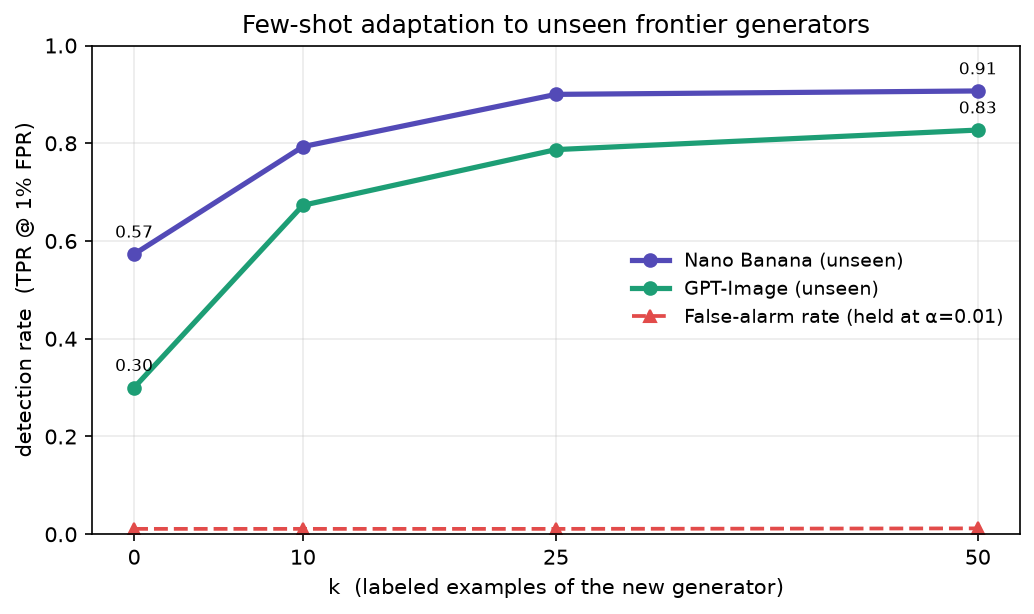
\includegraphics[width=0.72\textwidth]{figures/frontier_fewshot.png}
\caption{Few-shot adaptation to unseen frontier generators. Detection at a $1\%$
false-alarm rate rises sharply with a handful of labeled examples, while the
false-alarm rate stays at the $\alpha=0.01$ target.}
\label{fig:frontier}
\end{figure}

\subsection{Calibration behaviour}
The conformal threshold calibrated on training-domain reals transfers reasonably to
Chameleon (realized FPR $0.063$ at target $0.05$ for the probe). Under a strong
\emph{real-domain} shift (training on object/scene reals, testing on face reals) a
controlled experiment shows the guarantee breaking ($\text{FPR}\!:\,0.01\!\to\!0.27$)
and being restored to target ($\to\!0.01$) by recalibrating $\tau$ on unlabeled reals
from the new domain alone---no fake examples required. This separates what unlabeled
real data can fix (the false-alarm rate) from what it cannot (detection power, which
requires labeled fakes, as the few-shot curve shows).

\section{Discussion and limitations}
In-the-wild AI-image detection is unsolved; $\sim$0.90 AUC on Chameleon is competitive,
not perfect, and recall at a strict false-alarm budget remains modest. Robustness to a
new generator is obtained by few-shot adaptation on a small labeled set, which is the
realistic operating model as generators proliferate---not a permanent zero-shot
property. The frontier evaluation sets are small ($\sim$50 test images per generator),
so those point estimates carry wide intervals although the trends are stable across
seeds. The SigLIP backbone is Google's, used frozen and credited, as is standard
practice; the forensic stream, fusion head, calibration, provenance layer, data
assembly and evaluation are contributions of this work.

\section{Conclusion}
We built and deployed a calibrated, explainable AI-image detector with an honest
in-the-wild result ($0.90$ AUC on Chameleon), a measurable contribution from
physics-motivated forensic features, and a demonstrated few-shot recipe for adapting to
brand-new generators while holding the false-alarm rate at target. The system is
available as a public, interactive demo.

\begin{thebibliography}{9}
\bibitem{aide} S.~Yan et al. \emph{A Sanity Check for AI-Generated Image Detection.} ICLR 2025.
\bibitem{univfd} U.~Ojha et al. \emph{Towards Universal Fake Image Detectors that Generalize Across Generative Models.} CVPR 2023.
\bibitem{siglip} X.~Zhai et al. \emph{Sigmoid Loss for Language Image Pre-Training (SigLIP).} ICCV 2023.
\bibitem{calibrated} \emph{Your AI-Generated Image Detector Can Secretly Achieve SOTA Accuracy, If Calibrated.} arXiv:2602.01973, 2026.
\bibitem{conformal} \emph{Test-time Recalibration of Conformal Predictors under Distribution Shift Based on Unlabeled Examples.} arXiv:2210.04166, 2022.
\bibitem{nanobanana} J.~Zuo et al. \emph{Is Nano Banana Pro a Low-Level Vision All-Rounder? A Comprehensive Evaluation.} arXiv:2512.15110, 2025.
\bibitem{gptimgeval} Z.~Yan et al. \emph{GPT-ImgEval: A Comprehensive Benchmark for Diagnosing GPT-4o in Image Generation.} arXiv:2504.02782, 2025.
\bibitem{dalle3} J.~Betker et al. \emph{Improving Image Generation with Better Captions (DALL$\cdot$E 3).} OpenAI, 2023.
\bibitem{fakeorjpeg} \emph{Fake or JPEG? Revealing Common Biases in Generated Image Detection Datasets.} arXiv:2403.17608, 2024.
\end{thebibliography}

\end{document}
